\documentclass[a4paper, 12pt]{report}

% Adapté du tempate TER-M1 de l'Université de Paris

%%%%%%%%%%%%
% Packages %
%%%%%%%%%%%%

\usepackage[french]{babel}
%\usepackage{hyperref}
\usepackage[noheader]{packages/sleek}
\usepackage{packages/sleek-title}
\usepackage[french]{packages/sleek-theorems}
\usepackage{packages/sleek-listings}
\usepackage{tikz}
\usepackage[french,lined]{algorithm2e}	
\usepackage{pdfpages}
\usepackage{graphicx}
\graphicspath{ {./images/} }

\SetKwInput{KwResult}{R\'esultat}
\SetKw{KwInput}{Entr\'ees}
%%%%%%%%%%%%%%
% Title-page %
%%%%%%%%%%%%%%

\logo{./resources/img/logo_science.png}
\institute{Sorbonne Université}
\faculty{Master ANDROIDE}
\title{Titre du rapport}
\subtitle{UE de projet M1}
\author{Alessia \textsc{Loi} -- Dorian \textsc{LANCELIN}}
\date{2022}



%%%%%%%%%%%%%%%%https://www.overleaf.com/project/6012bd305aee4065605e8f1d
% Bibliography %
%%%%%%%%%%%%%%%%

\addbibresource{./resources/bib/references.bib}

%%%%%%%%%%
% Others %
%%%%%%%%%%

\lstdefinestyle{latex}{
    language=TeX,
    style=default,
    %%%%%
    commentstyle=\ForestGreen,
    keywordstyle=\TrueBlue,
    stringstyle=\VeronicaPurple,
    emphstyle=\TrueBlue,
    %%%%%
    emph={LaTeX, usepackage, textit, textbf, textsc}
}

\FrameTBStyle{latex}

\def\tbs{\textbackslash}

%%%%%%%%%%%%
% Document %
%%%%%%%%%%%%

\begin{document}
    \maketitle
    \romantableofcontents

    \chapter{Introduction}

    -On cherche à trouver des outils permettant à des robots avec une mémoire très limitée d'apprendre à réaliser une tâche par observation des mouvements d'autres robots au mêmes spécifications.
    
    - On considèrera que les robots ont des moyens de communication limités voire inexistant si possible.
    
    - En utilisant des agents au comportement prédéfini, les experts, capables de réaliser au mieux la tâche envisagée, on arrive toujours à observer une convergeance vers le comportement de l'expert dans les cas où l'apprentissage se fait uniquement dans le sens expert-apprenant.
    Dans certains cas particuliers, des méthodes explorées permettent a l'apprentissage apprenant-apprenant d'accélerer cette convergeance. 
    
    Ce projet a été encadré par messieurs Nicolas Bredeche et Stéphane Doncieux.  
    
    L'ensemble des codes utilisé afin d'obtenir les résultats décrit dans le document suivant sont disponible sur notre dépôt \href{https://github.com/aerrynn/M1_Projet_ASIRE}{github}. 

    \chapter{État de l'art}
    Un chapitre dédié à l'état de l'art doit décrire les concepts et méthodes déjà existant(e)s, en lien avec le travail que vous avez réalisé.
    
    \chapter{Contribution}
   
    \section{Choix de l'expérimentation : La tâche de fourragement}
    Dans le but d'évaluer la capacité d'apprentissage par comportement de notre essaim de robots, on a reproduit l'expérience de fourragement et simulée à l'aide de pyRoborobo.
    L'évaluation en elle-même se fait sur la quantité d'objets capturés par un agent sur une fenêtre de temps donnée (sliding window). On considèrera qu'il n'y a pas de perte d'information lors du transfert, c'est à dire que l'apprenant est capable de voir tout ce que voit l'expert.
    On définit ainsi les paramètres de l'expérience :
    \begin{itemize}
    \item Taille de la population : 100
    \item Nombre d'experts : 10
    \item Nombre d'apprenants : 90
    \item Nombre d'objets : 100
    \item Taille de l'arène : 1400x800
    \item Taille des robots : 5x5
    \item Nombre de senseurs : 16
    \item Distance des senseurs : 16
    \item Durée d'une expérience : 20,000
    \item Nombre de répétion de l'expérience : 5
    \end{itemize}

Les différents experts suivent un comportement donné.
// Algo comportement 1 : sous forme de génome

// Algo comportement 2
L'objectif de ce comportement est d'éviter les obstacles (qu'ils soient des murs ou d'autres robots) tout en se focalisant sur le ramassage des objets dès que possible.

	\section{Méthodes explorées}
	
	\section{Méthode de transmission}
	blah
	\section{Méthode par mimétisme}
	blash
	\subsection{Apprentissage ad-hoc}
	Dans un premier temps, on décide d'évaluer l'apprentissage par mimétisme en donnant aux apprenants une mémoire extensible et en déterminant le comportement des agents non-experts de la manière suivante :
	

	\begin{algorithm}[H]
		\KwInput{une observation $o$}\;
		\KwResult{l'action à effectuer $a$ }
  		On cherche l'observation $o'$ présente dans la mémoire telle que la distance $o$-$o'$ soit minimale\;
		L'observation $o'$ étant stockée avec une action $a'$ associée : $a$ $\leftarrow$ $a'$ \;
  		return $a$\;
	\end{algorithm}
	
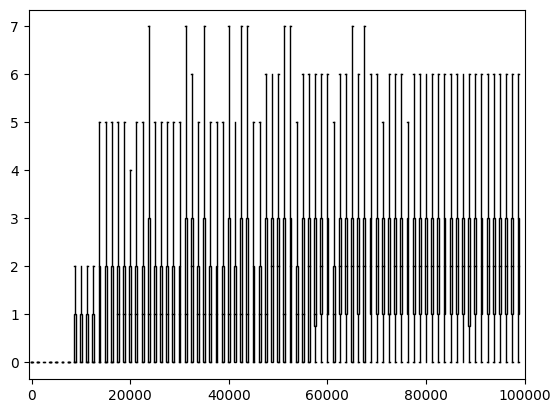
\includegraphics{learner_boxplot}
	
	La première remarque que l'on peut faire sur cette méthode d'apprentissage est qu'au délà d'être coûteuse en mémoire (// nbre de comportements appris à un temps t), la simulation dure très longtemps du fait que les observations appartiennent à des segments continus compris entre 0 et 1.
	
	De plus, lorsqu'un apprenant apprend un comportement, celui-ci est toujours dans le rayon de perception de l'expert, ce qui entraine une perte de généralisation. Par exemple les situation où un agent se retrouve en face d'un objet sans qu'aucun autre agent ne soit détecté par ses senseurs ne peuvent être apprises.
	Pour palier à ce problème, dans un premier temps, on a fait le choix de ne transmettre que les informations des capteurs frontaux.
	Lorsque l'on ajoute l'apprentissage inter-apprenants, on observe rapidement à un problème : un agent non-expert peut apprendre un mauvais comportement et l'on a -pour l'instant - aucun moyen de filtrer ou d'éliminer ces comportements sub-optimaux.
	
	\subsection{apprentissage ad-hoc avec discrétisation des entrées}
	Afin d'adapter la méthode ad-hoc au domaine de la robotique en essaim, et donc de limiter la mémoire nécessaire, on a essayé de discrétiser les entrer. Une telle méthode a plusieur avantage : elle réduit le domaine des observations $$nombre d'intervalles^{nombre de senseurs}*2^{nombre de senseurs de typage} $$ et permet de hasher ces dernière pour accéder plus efficacement aux comportements.
	Pour cette version, le comportement des apprenants suit les règles suivante :
	

\begin{algorithm}[H]
	\KwInput{une observation $o$}\;
	\KwResult{l'action à effectuer $a$ }
	$o'$ $\leftarrow$ Discrétiser($o$)\;
	\If{o' est une clé du dictionnaire $mémoire$}								
	{\Return mémoire[$o'$]}
	\Return mouvement par défaut\;
\end{algorithm}
	
	
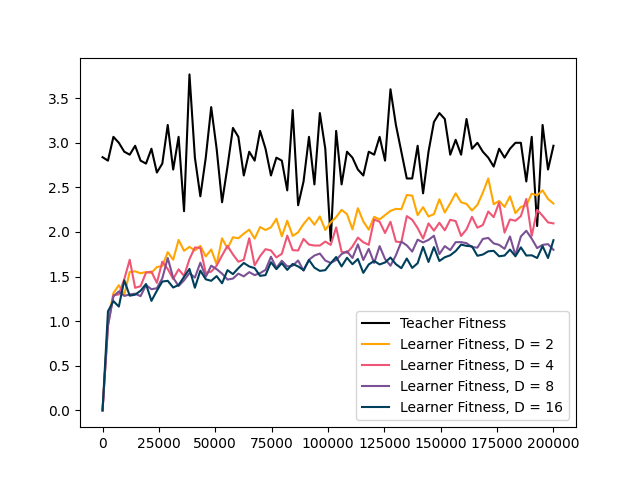
\includegraphics{averageComparisons}


	Par ces analyse, on remaque que lorsque le nombre d'intervalles de discrétisation augmente, la convergeance est de plus en plus lente ce qui s'explique par le plus grand nombre de comportements à apprendre.
	 Cette supposition est confirmé par la quantité de mouvements appris en fonction du nombre d'intervalles de discrétisations.
	 
	 
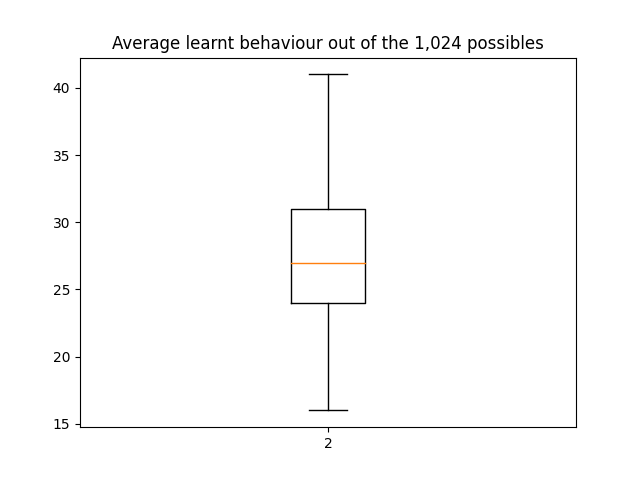
\includegraphics{averageLearntBehaviourD2}
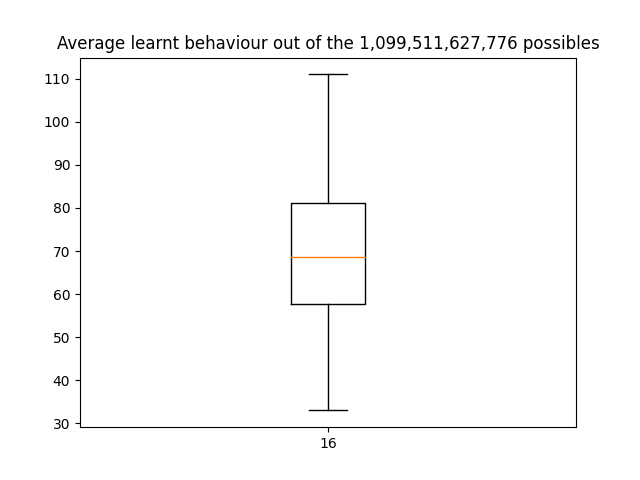
\includegraphics{averageLearntBehaviourD16}
	
	En revanche si le nombre d'intervalles est insuffisant, une partie du comportement de l'expert peut être perdue. Par exemple si un expert adopte trois comportements différents en fonction de la valeur du senseur 1, une discrétisatione en deux intervalles (respectivement [0,0.5], ]0.5,1]) ne permettrait pas l'apprentissage exact de ce comportement.
	
	Pour implémenter la propagation, il suffit de modifier la règle d'apprentissage de la manière suivante :
	
	%// Pseudocode
\begin{algorithm}[H]
	Lors de la réception d'un message $m$\;
	$o$,$a$ $\leftarrow$ $m$
	\If {$a\neq$ action par défaut}{$o'\leftarrow$discrétiser($o$)
	\If {$o'$ n'est pas une clé de du dictionnaire $mémoire$}{$mémoire$[$o'$] $\leftarrow a$}}
\end{algorithm}
	
	
	\textbf{N.B.}Pour les tests, on a fait le choix de définir le mouvement par défaut comme (0.5, 0.05), c'est à dire de continuer tout droit, mais avec un léger déplacement vers la droite pour éviter de se coincer.
	
	\subsection{Apprentissage ad-hoc avec PPV}
	Une autre option envisagée pour réduire la demande en mémoire de notre algorithme est de toujours exécuter l'action de la mémoire dont l'observation est la plus proche de l'observation actuelle.
	De plus afin de limiter le nombre de points insérés dans la mémoire, on a implémenté l'algorithme suivant :
	
\begin{algorithm}[H]
	\SetAlgoLined
	Lors de la réception d'un message $m$\;
	$o$,$a$, $w$ $\leftarrow$ $m$
	On cherche le couple ($o'$, $a'$) tel que la distance $o-o'$ soit minimale\;
	\If{$a\neq a'$}{On ajoute le tuple ($o$, $a$, 1) à la mémoire}{On modifie $o$ de la manière suivante\;
	$o'\leftarrow$ ( $ \frac{o'* w + o}{w+1}$}
\end{algorithm}
	
 // Graph + Eval
	
	\subsection{Apprentissage sur un réseau de Neurone par Backpropagation}
	Pour remédier aux différents problèmes remarqués dans les méthodes ad-hoc, on a essayé d'appliquer l'apprentissage par mimétisme sur un réseau neuronal. Ainsi, la présence d'un agent sur un senseur donné devrait disparaitre lors de la généralisation.
	Un problème s'est néanmoins présenter : certaines observations sont beaucoups plus représentées que d'autres
	
	//Figure représentative :
	
	Pour palier à cela, on a donc renforcé l'apprentissage en pondérant la rétropropagation lors de l'apprentissage en fonction de la distance à l'objectif.
	
	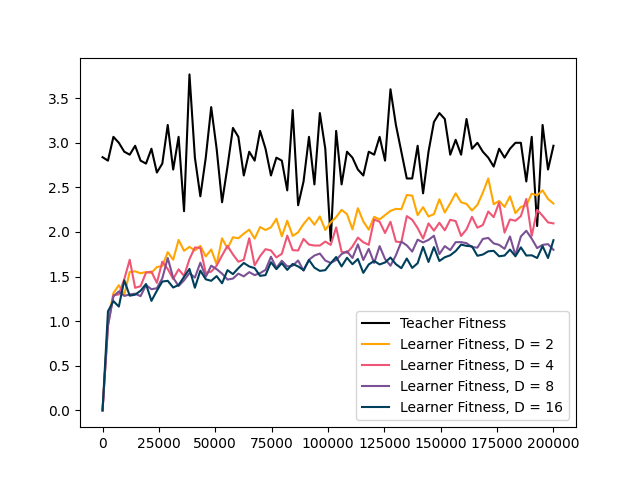
\includegraphics{averageComparisons}
	
Cette méthode est, comme attendu, plus lente que la version ad-hoc. En revanche elle semble suivre une croissance continue. Il serait envisageable de poursuivre l'experience jusqu'à la stabilisation de la population.
	
	
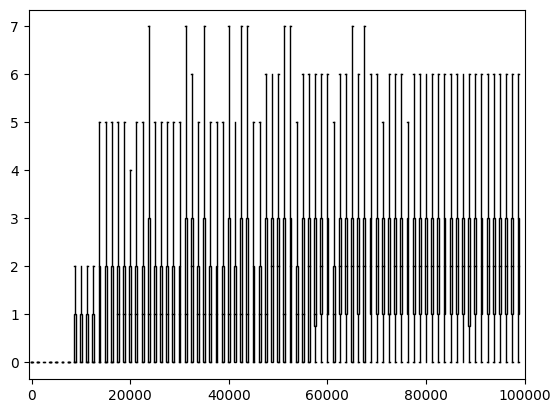
\includegraphics{learner_boxplot}
	
	//Evaluation 

    \section{Bibliographie}
//TODO
Nous recommandons l'usage de \href{https://fr.wikipedia.org/wiki/BibTeX}{BibTeX} pour la gestion de la bibliographie. Ajoutez les entrées correspondant à vos références dans le fichier \verb+resources/bib/references.bib+. Vous pouvez obtenir les entrées BibTeX sur \href{https://scholar.google.com}{Google Scholar} ou \href{https://dblp.uni-trier.de}{DBLP}. La commande \verb+\cite+ vous permet de citer une (ou plusieurs) référence(s) dans le document, par exemple \cite{pakin2020comprehensive,RusselNorvig}.

\chapter{Conclusion}
Pour la poursuite de notre projet, nous devrions optimiser les différents codes pour permettre des expériences plus représentatives, mais surtout pouvoir comparer nos résultats avec les algorithmes "state of the art"

    %\printbibliography

    \appendix

    \chapter{Cahier des charges}
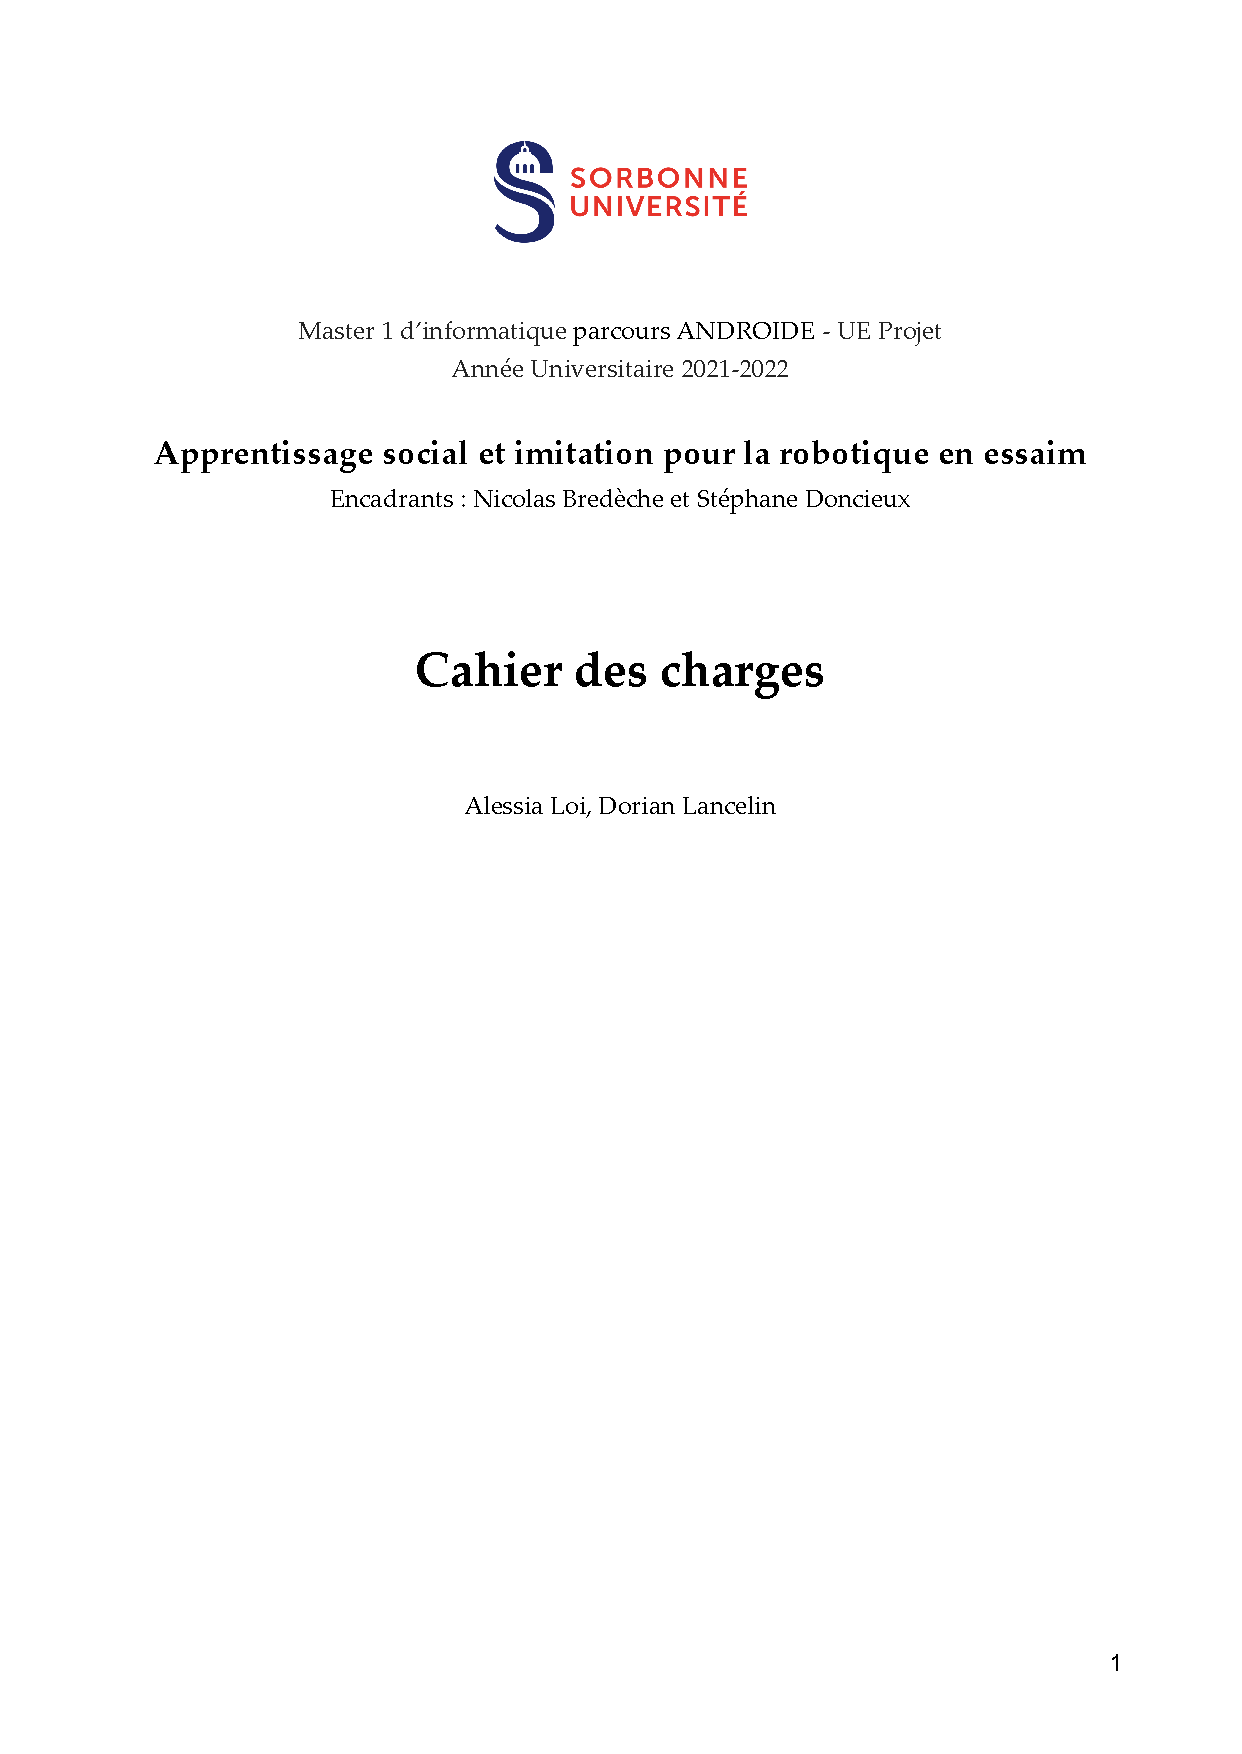
\includepdf[scale = 0.8,nup=2x2, pages=1-4]{CDC.pdf}
     \chapter{Manuel utilisateur}
	Un manuel utilisateur permettant la prise en main de votre code. 

\end{document}
